\chapter{Results and Discussions}\label{ch:results}
% This MUST remain the penultimate main chapter under the supplied guideline.
\section{Measured Results}
All numbers in this chapter are read from the committed scores file (\url{results/rop/v3/v3_scores.json}, commit \texttt{b827cce}) and the report-data file derived from it; every figure is drawn by a committed script from those files. Pooled numbers average both seeds; intervals are 95\% infant-clustered bootstrap intervals.

\subsection{The nine models}
Table~\ref{tab:headline} gives the headline metrics and Figure~\ref{fig:compare} the QWK of every model with its interval, in cross-validation and at the held-out hospital. The pre-registered selection rule (cross-validation QWK) selects model~B, DINOv2, at 0.825; the baseline scores 0.816. Across the nine models cross-validation QWK spans 0.794 to 0.825; at the held-out hospital the eye-level QWK values span 0.744 (F) to 0.776 (I) and every one lies inside the baseline's interval (0.680--0.822).
\begin{table}[htbp]
\caption{Headline metrics of the nine models (pooled over two seeds)}\label{tab:headline}
\begingroup\TightTable\small
\begin{tabularx}{\textwidth}{@{}p{34mm}YYYYYY@{}}\toprule
Model & CV QWK (95\% CI) & CV acc. & CV macro-F1 & Eye QWK at new hospital (95\% CI) & Eye acc. & Eye macro-F1\\\midrule
A RETFound-Green & 0.794 (0.664--0.915) & 0.758 & 0.643 & 0.774 (0.707--0.828) & 0.632 & 0.563\\
B DINOv2 & \textbf{0.825} (0.737--0.911) & 0.766 & 0.653 & 0.756 (0.679--0.821) & 0.630 & 0.566\\
C EfficientNet (baseline) & 0.816 (0.713--0.916) & 0.788 & 0.656 & 0.760 (0.680--0.822) & 0.624 & \textbf{0.573}\\
D DINOv2 + exam loss & 0.797 (0.699--0.909) & \textbf{0.802} & 0.661 & 0.746 (0.671--0.810) & 0.609 & 0.542\\
E Ensemble A+B+C & 0.821 (0.708--0.927) & 0.787 & \textbf{0.664} & 0.770 (0.697--0.827) & \textbf{0.639} & 0.568\\
F DINOv2 + adaptation$^\dagger$ & 0.812 (0.704--0.915) & 0.760 & 0.644 & 0.744 (0.665--0.812) & 0.624 & 0.551\\
G DINOv2 at 518 px & 0.814 (0.706--0.915) & 0.764 & 0.647 & 0.767 (0.697--0.827) & 0.626 & 0.551\\
H DINOv2, v4 pool & 0.813 (0.707--0.914) & 0.765 & 0.646 & 0.750 (0.674--0.814) & 0.620 & 0.556\\
I DINOv2, v4 pool + recipe & 0.821 (0.727--0.912) & 0.750 & 0.618 & \textbf{0.776} (0.705--0.834) & 0.633 & 0.560\\
\bottomrule
\end{tabularx}\endgroup
\par\small $^\dagger$ model F saw the held-out hospital's photographs, without labels, during training; its new-hospital numbers are transductive.
\end{table}
\begin{figure}[htbp]
\centering
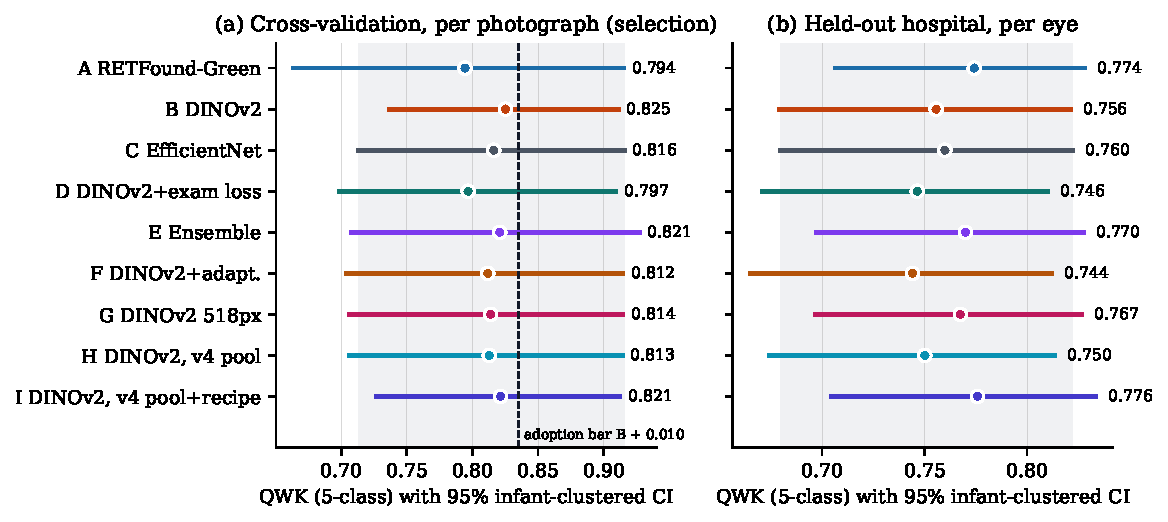
\includegraphics[width=\textwidth]{fig_compare.pdf}
\caption{QWK of the nine models with 95\% infant-clustered intervals; the shaded band is the baseline's interval, the dashed line the v4 adoption bar (B $+$ 0.010)}\label{fig:compare}
\end{figure}

\subsection{The v4 round: data audit and recipe}\label{sec:v4results}
The audit of Section~\ref{sec:v4design} found 585 of the 4{,}285 Ostrava frames below their camera's quality thresholds (429 for sharpness, 108 too dark, 108 too bright; a frame can fail more than one test); 584 left the training candidates and one was kept by the two-frame floor. Within the caps, 439 of v3's 715 Ostrava training rows were replaced by 418 sharper frames, and the v4 training pool holds 3{,}083 photographs against 3{,}112 (stage~1: 497 against 515). Of 109 photograph pairs within dHash distance 4, the pixel check confirmed 72 as true duplicates; the cross-fold rule removed 8 photographs, all already among the 14 exact duplicates, so in practice it changed no trained-on photograph, and 14 pairs with different labels went to the clinician list.

Table~\ref{tab:selection} gives the adoption rule as scored. Neither v4 model reached the margin: I is 0.004 and H 0.012 below B in cross-validation, where $+0.010$ was required, although both passed the LOSO guard. \textbf{Model B stays selected.} The paired intervals confirm it: I$-$B is $-0.004$ ($-0.015$ to $+0.007$) and H$-$B $-0.013$ ($-0.031$ to $+0.009$), both wholly below the bar.
\begin{table}[htbp]
\caption{The v4 adoption rule (Amendment 5c) as scored; differences of the four-decimal selection-table values}\label{tab:selection}
\begingroup\TightTable\small
\begin{tabularx}{\textwidth}{@{}p{30mm}YYYYYYp{18mm}@{}}\toprule
Model & CV QWK & $\Delta$ vs B & Needs & Mean LOSO & $\Delta$ vs B & Needs & Outcome\\\midrule
I DINOv2, v4 pool + recipe & 0.821 & $-0.0038$ & \mbox{$\ge +0.010$} & 0.839 & $+0.0054$ & \mbox{$\ge -0.010$} & not adopted\\
H DINOv2, v4 pool & 0.813 & $-0.0124$ & \mbox{$\ge +0.010$} & 0.842 & $+0.0085$ & \mbox{$\ge -0.010$} & not adopted\\
B DINOv2 & 0.825 & & & 0.834 & & & \textbf{stays}\\
\bottomrule
\end{tabularx}\endgroup
\end{table}

Table~\ref{tab:loso} and Figure~\ref{fig:loso} give the leave-one-source-out folds. The three models are close on each held-out hospital; the Ostrava fold has intervals 0.40--0.45 wide because its 4{,}285 photographs come from only 148 infants, and I is 0.020 below B when Shenzhen is held out. The ROP-VL fold trains with no stage-4/5 photograph and scores none of them correctly, which is why stage~4/5 must come from more than one source before any model can be trusted on it at a new hospital.
\begin{table}[htbp]
\caption{Leave-one-source-out QWK (5-class) with 95\% infant-clustered CI, both seeds pooled}\label{tab:loso}
\begingroup\TightTable\small
\begin{tabularx}{\textwidth}{@{}p{38mm}p{10mm}YYYp{14mm}@{}}\toprule
Model & Pool & Shenzhen held out & Ostrava held out & ROP-VL held out & Mean\\\midrule
B DINOv2 & v3 & 0.962 (0.953--0.971) & 0.740 (0.398--0.845) & 0.799 (0.771--0.827) & 0.834\\
H DINOv2, v4 pool & v4 & 0.960 (0.950--0.969) & 0.766 (0.452--0.858) & 0.801 (0.774--0.824) & 0.842\\
I DINOv2, v4 pool + recipe & v4 & 0.942 (0.926--0.956) & 0.779 (0.471--0.875) & 0.796 (0.768--0.820) & 0.839\\
\bottomrule
\end{tabularx}\endgroup
\end{table}
\begin{figure}[htbp]
\centering
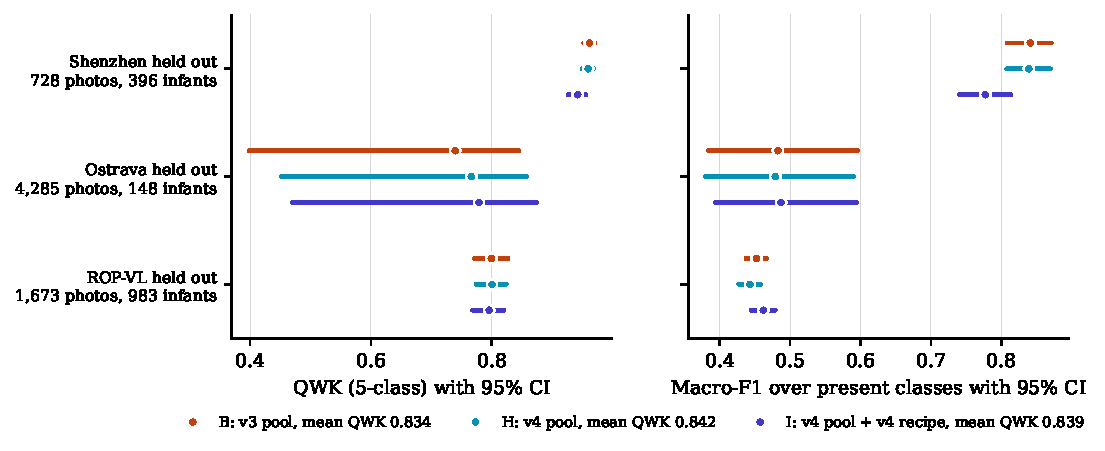
\includegraphics[width=\textwidth]{fig_loso.pdf}
\caption{Leave-one-source-out folds of models B, H and I: QWK and macro-F1 on every photograph of the held-out hospital}\label{fig:loso}
\end{figure}

At the held-out hospital, which does not enter the rule, model~I scored best of all nine models (0.776, 95\% CI 0.705--0.834): I$-$B is $+0.020$ ($+0.003$ to $+0.041$) and I$-$H $+0.026$ ($+0.006$ to $+0.046$), while H$-$B is $-0.005$ ($-0.015$ to $+0.003$). The gain is in QWK only (eye-level macro-F1 I$-$B $-0.005$, $-0.057$ to $+0.033$) and comes from stage~2 (recall 0.60 against 0.55) and from fewer stage-1 eyes called normal. It is descriptive: the development half has now been examined for nine models, and the gain is a quarter of the 0.08 difference that even the locked half can detect. Model~I is also the best calibrated as trained (Section~\ref{sec:calib}).

The cost of the v4 changes shows in cross-validation macro-F1 (I$-$B $-0.035$, $-0.053$ to $-0.001$) and in AP-ROP recall, which falls from 0.389 (B) to 0.306 (H) and 0.269 (I). The fall sits entirely in fold~0: 470 of its 476 AP-ROP validation photographs are frames of one Ostrava infant, scored by fold-0 models that train on no Ostrava AP-ROP frame. There AP-ROP recall is 0.246, 0.142 and 0.101 for B, H and I (the two seeds of B alone differ by 0.160), while on folds 1--4, whose AP-ROP photographs come from ROP-VL infants, the three models reach 0.866, 0.859 and 0.835. Both pools hold the same 168 AP-ROP training photographs. The drop is therefore a label-unit artefact: one examination label stamped on 470 near-identical frames, read slightly differently by models whose other training frames changed.

\subsection{Paired differences}
Figure~\ref{fig:contrasts} shows the pre-registered paired contrasts. At the held-out hospital, A$-$C is $+0.014$ (95\% CI $-0.012$ to $+0.048$), B$-$C is $-0.004$ ($-0.038$ to $+0.030$), E$-$C is $+0.010$ ($-0.012$ to $+0.040$), G$-$B is $+0.012$ ($-0.005$ to $+0.032$) and H$-$B is $-0.005$ ($-0.015$ to $+0.003$): these intervals cross zero. Two contrasts exclude zero below it, both small: D$-$A is $-0.028$ ($-0.048$ to $-0.011$) and F$-$B is $-0.011$ ($-0.022$ to $-0.002$). Three lie above it: I$-$B $+0.020$ ($+0.003$ to $+0.041$), I$-$H $+0.026$ ($+0.006$ to $+0.046$) and A$-$B $+0.018$, whose lower bound is 0.000. In cross-validation E$-$A is $+0.026$ ($+0.008$ to $+0.045$); every other cross-validation contrast crosses zero.
\begin{figure}[htbp]
\centering
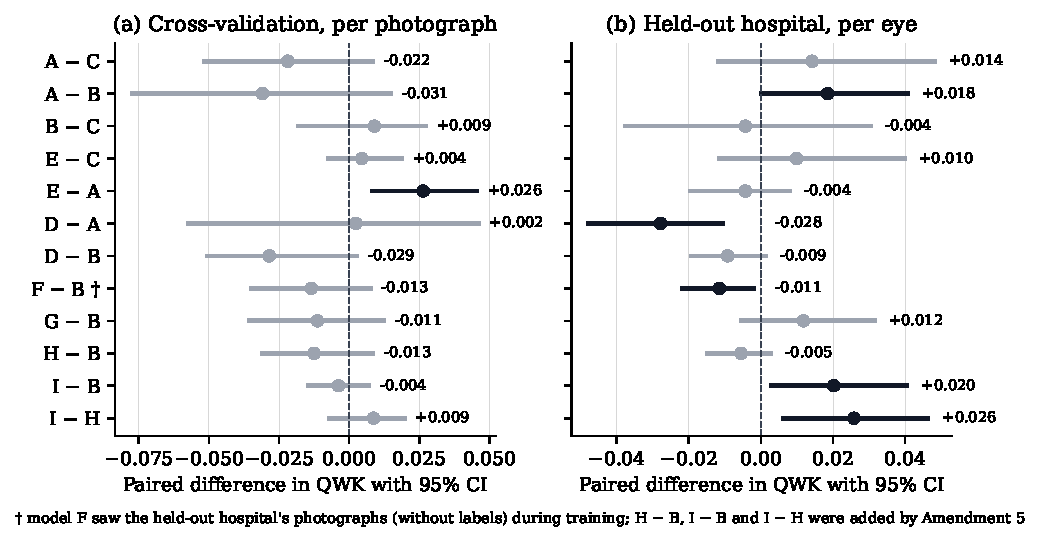
\includegraphics[width=\textwidth]{fig_contrasts.pdf}
\caption{Paired differences in QWK between models, both models scored on the same resampled infants; a bar crossing zero is a tie; H$-$B, I$-$B and I$-$H were added by Amendment~5}\label{fig:contrasts}
\end{figure}

\subsection{Stage by stage}
Figure~\ref{fig:stagerecall} gives recall by stage and Table~\ref{tab:perclass} the per-class metrics of the selected model. Stage~1 is where the transformers differ from the baseline: at the held-out hospital, stage-1 eye recall is 0.52 for A, 0.51 for B, G and I and 0.50 for H, against 0.40 for C; in cross-validation 0.57--0.61 for A, B, F, G and H against 0.50 for C. Model~I is the exception in cross-validation (0.49): its recipe, not its pool, costs stage-1 recall there, since H shares the pool and keeps 0.57. The baseline is better on AP-ROP at both levels, and the models are otherwise within a few points of one another.
\begin{figure}[htbp]
\centering
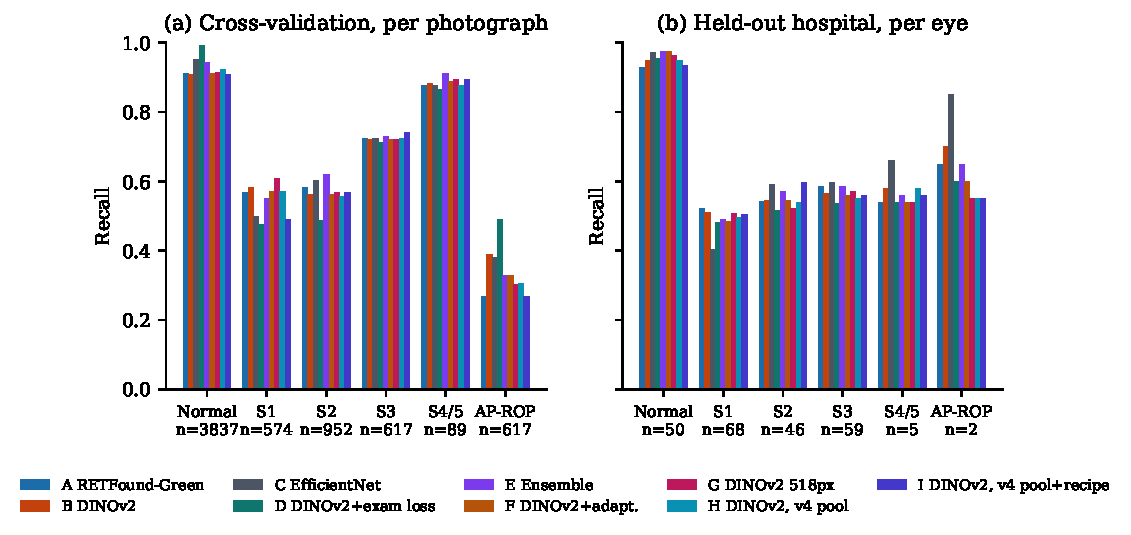
\includegraphics[width=\textwidth]{fig_stage_recall.pdf}
\caption{Recall by stage for every model, in cross-validation and at the held-out hospital}\label{fig:stagerecall}
\end{figure}
\begin{table}[htbp]
\caption{Per-class metrics of model B (DINOv2), pooled over seeds}\label{tab:perclass}
\begingroup\TightTable\small
\begin{tabularx}{\textwidth}{@{}p{18mm}YYYYY|YYYYY@{}}\toprule
 & \multicolumn{5}{c|}{Cross-validation, per photograph} & \multicolumn{5}{c}{Held-out hospital, per eye}\\
Stage & $n$ & Prec. & Recall & F1 & AUC & $n$ & Prec. & Recall & F1 & AUC\\\midrule
Normal & 3,837 & 0.96 & 0.91 & 0.93 & 0.98 & 50 & 0.62 & 0.95 & 0.75 & 0.95\\
Stage 1 & 574 & 0.30 & 0.58 & 0.40 & 0.82 & 68 & 0.61 & 0.51 & 0.55 & 0.72\\
Stage 2 & 952 & 0.58 & 0.56 & 0.57 & 0.90 & 46 & 0.67 & 0.55 & 0.60 & 0.83\\
Stage 3 & 617 & 0.79 & 0.72 & 0.75 & 0.94 & 59 & 0.87 & 0.57 & 0.68 & 0.88\\
Stage 4/5 & 89 & 0.67 & 0.88 & 0.76 & 0.96 & 5 & 0.76 & 0.58 & 0.65 & 0.68\\
AP-ROP & 617 & 0.70 & 0.39 & 0.50 & 0.83 & 2 & 0.09 & 0.70 & 0.16 & 0.97\\
\bottomrule
\end{tabularx}\endgroup
\end{table}

\subsection{Confusion matrices}
Figure~\ref{fig:confusion} shows where the errors are for the selected model. In cross-validation, 332 normal photographs are called stage~1 and 251 stage-2 photographs are called stage~1; AP-ROP photographs are spread over stages 1 to 3. At the held-out hospital, per eye, 24 of 68 stage-1 eyes are called normal and 11 of 46 stage-2 eyes are called stage~1; serious errors (two or more stages) are rare. Model~I's matrices (Appendix~\ref{app:tests}) call 22.4 stage-1 eyes normal on average and keep more stage-2 eyes in their own class (27.4 against 25.1). The baseline's matrices (Appendix~\ref{app:tests}) show the same 24 stage-1 eyes called normal per eye, and in cross-validation fewer normal photographs called stage~1 (163 against 332) at the cost of lower stage-1 recall.
\begin{figure}[htbp]
\centering
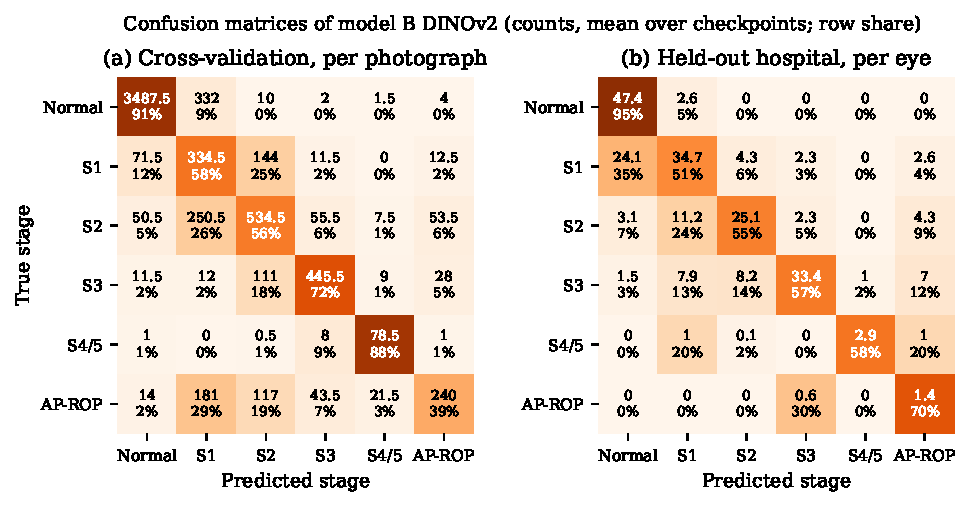
\includegraphics[width=\textwidth]{fig_confusion_B.pdf}
\caption{Confusion matrices of model B: counts (mean over checkpoints) and share of each true-stage row}\label{fig:confusion}
\end{figure}

\subsection{Detecting any ROP, calibration and the operating point}\label{sec:calib}
Figure~\ref{fig:curves} gives the ROC and precision--recall curves for ROP against normal per eye: AUC 0.935--0.944 for every model, and average precision 0.98 (prevalence 0.78). Figure~\ref{fig:calibration} gives the reliability curves: models A--H are over-confident at the new hospital (ECE 0.14--0.18), and model~I, trained with the weight average and stronger label smoothing, is close to the diagonal (ECE 0.061). The temperature fitted on cross-validation (0.62--0.94, i.e.\ sharpening for every model) makes every model worse there (ECE 0.20--0.24, model~I 0.196). The pre-registered any-ROP threshold, set to 90\% sensitivity on cross-validation, reaches 64--68\% sensitivity at the held-out hospital for every model, at 100\% specificity; the threshold does not transfer.
\begin{figure}[htbp]
\centering
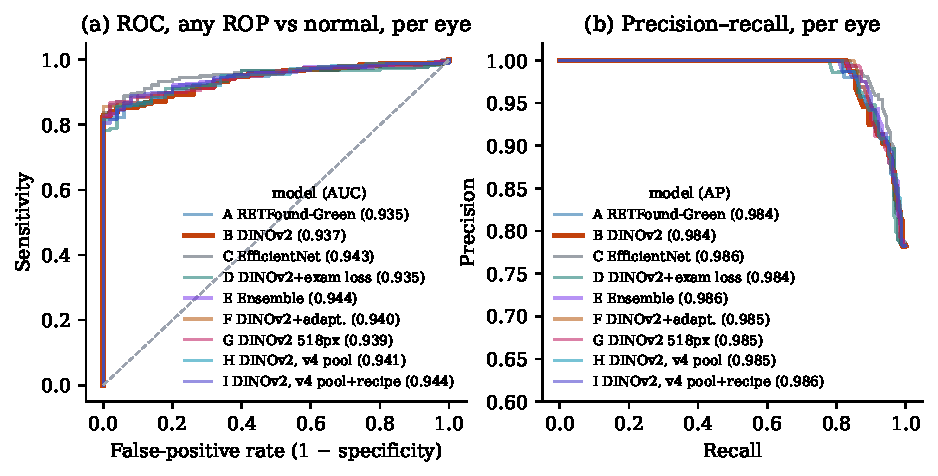
\includegraphics[width=\textwidth]{fig_curves.pdf}
\caption{Any-ROP detection at the held-out hospital, per eye: (a) ROC curves; (b) precision--recall curves}\label{fig:curves}
\end{figure}
\begin{figure}[htbp]
\centering
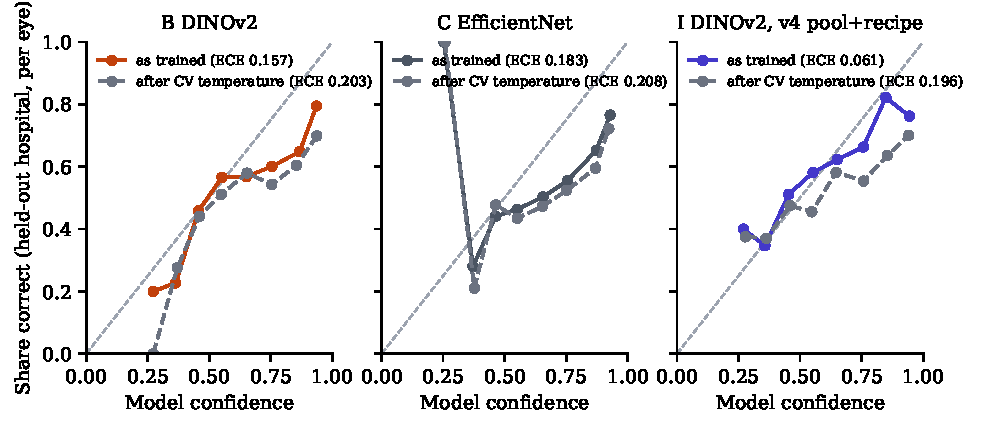
\includegraphics[width=\textwidth]{fig_calibration.pdf}
\caption{Reliability curves per eye at the held-out hospital for models B, C and I, as trained and after the cross-validation temperature}\label{fig:calibration}
\end{figure}

\subsection{Results by hospital unit, and the one real gain}
Figure~\ref{fig:units} scores each training hospital at its own unit in cross-validation. At the Ostrava examination level, model~D (trained one session at a time) scores 0.846 against 0.701 for model~B, the same encoder trained per photograph, and 0.775 for the baseline; cleaning Ostrava's frames (models H and I) gives 0.710 and 0.712, so sharper frames do not do what the examination-level loss does. A post-hoc paired bootstrap on the 342 Ostrava examinations (148 infants, 64 diseased examinations from 18 infants) gives D$-$B $+0.145$ (95\% CI $+0.094$ to $+0.257$) in QWK and $+0.214$ in macro-F1; D$-$C is $+0.071$ ($+0.015$ to $+0.230$). This contrast was not pre-registered and rests on 18 diseased infants, and model~D also gives Ostrava a larger share of training steps (36\% against 22\%), which is a confound to be disclosed.
\begin{figure}[htbp]
\centering
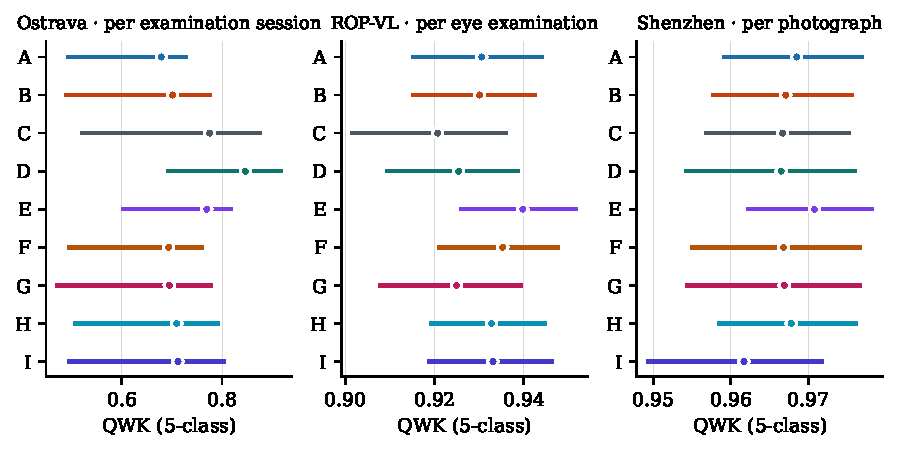
\includegraphics[width=\textwidth]{fig_units.pdf}
\caption{Cross-validation QWK of every model at each hospital's own unit: Ostrava per examination session, ROP-VL per eye examination, Shenzhen per photograph}\label{fig:units}
\end{figure}

\subsection{Inference time}\label{sec:p5}
\PFIVETEXT

\subsection{Training behaviour, folds and run times}
Figure~\ref{fig:training} shows the training loss and the held-out macro-F1 by epoch, averaged over the ten runs of each arm; all arms converge smoothly within 20 epochs with no sign of over-fitting of the held-out fold. Model~I's loss sits higher by construction (label smoothing 0.10 against 0.05), and its held-out macro-F1 rises later because it is measured on the weight average, which early in training still carries most of the pre-trained weights. Figure~\ref{fig:folds} shows the score of each fold: fold~0, which holds 476 of the 617 AP-ROP photographs, is the hardest for every model (QWK 0.59--0.74), and the seeds differ by up to 0.08 on it. Table~\ref{tab:timing} gives the run times from the Kaggle logs.
\begin{figure}[htbp]
\centering
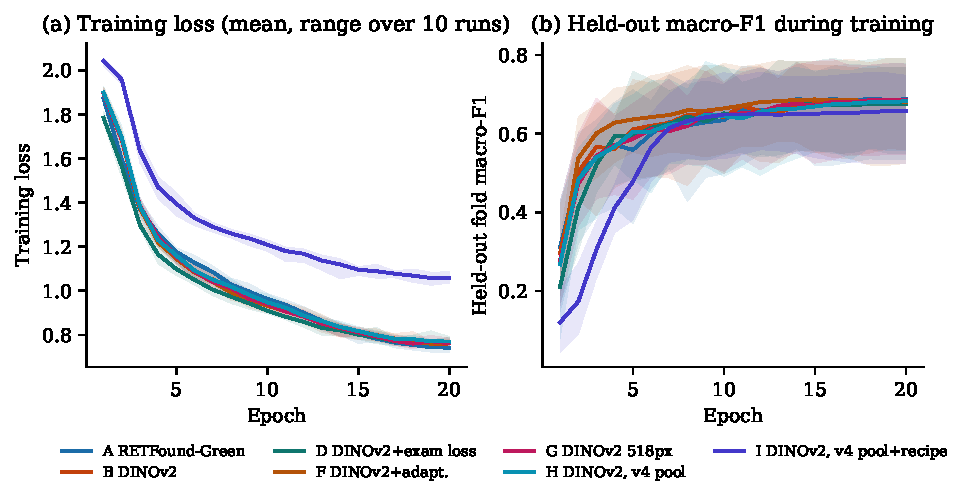
\includegraphics[width=\textwidth]{fig_training.pdf}
\caption{Training curves of the transformer arms: mean over ten runs with the range shaded}\label{fig:training}
\end{figure}
\begin{figure}[htbp]
\centering
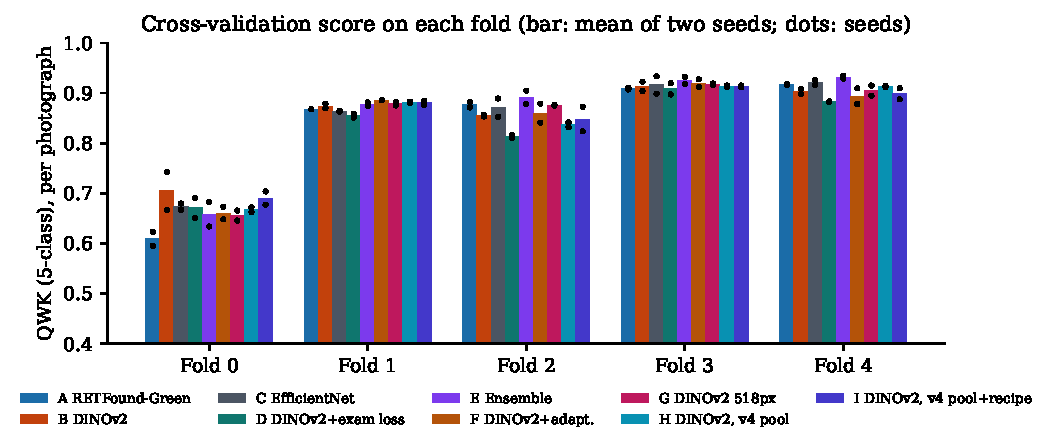
\includegraphics[width=\textwidth]{fig_folds.pdf}
\caption{Cross-validation QWK on each fold, by model and seed}\label{fig:folds}
\end{figure}
\begin{table}[htbp]
\caption{Training time on a Kaggle T4 GPU, from the kernel logs (20 epochs per fold; F and G train the five CV folds only; for H and I the session column counts the five CV folds and the site fold, without their two LOSO folds)}\label{tab:timing}
\begingroup\TightTable\small
\begin{tabularx}{\textwidth}{@{}p{34mm}YYYY@{}}\toprule
Model & Photos/s & Min per fold & Min per session (5 folds + site) & Kernels\\\midrule
A RETFound-Green & 39 & 32 & 187--189 & one kernel per seed\\
B DINOv2 & 32 & 33 & 191--200 & one kernel per seed\\
D DINOv2 + exam loss & 29 & 33 & 188--193 & one kernel per seed\\
F DINOv2 + adaptation & 14 & 62 & 302--316 & two kernels per seed\\
G DINOv2 at 518 px & 19 & 58 & 287--294 & two kernels per seed\\
H DINOv2, v4 pool & 31 & 34 & 196--202 & two per seed (CV; site + 2 LOSO)\\
I DINOv2, v4 pool + recipe & 32 & 35 & 191--216 & two per seed (CV; site + 2 LOSO)\\
\bottomrule
\end{tabularx}\endgroup
\end{table}

\section{Verification of Project Requirements}
\noindent Table~\ref{tab:verification} links each requirement to its test and evidence.
\begin{table}[htbp]
\caption{Verification of project requirements}\label{tab:verification}
\begingroup\TightTable\small
\begin{tabularx}{\textwidth}{@{}p{8mm}YYYp{18mm}Y@{}}\toprule
ID & Requirement and criterion & Test & Actual result & Status & Evidence\\\midrule
R1 & Eye route: 1--16 photographs in, JSON out; errors as JSON & T1 & 200 with demo set; 413, 422, 400 cases covered & Met & \url{tests/test_eye_route.py}\\
R2 & Worst-view rule with AP-ROP as a form & T1 & Unit tests pass & Met & \url{webapp/inference.py}\\
R3 & PDF report with eye summary & T1 & Generated and validated & Met & \url{reports/}\\
R4 & One-command training with aligned saved predictions & T2 & 14 sessions collected; none rejected & Met & \url{results/rop/v3/runs/}\\
R5 & Scorer from saved predictions with reproduction check & T3 & Baseline reproduced to 3 dp; refuses otherwise & Met & \url{v3_scores.json}\\
R6 & Locked half never read & T3 & Guard and AST test pass & Met & \url{tests/test_v3_uda.py}\\
P1 & CV QWK $\ge0.80$ & T4 & 0.825 (0.737--0.911) & Met & Table~\ref{tab:headline}\\
P2 & Eye QWK at new hospital $\ge0.75$ & T5 & 0.756 (0.679--0.821); served configuration \DeployedQWK & Met & Table~\ref{tab:headline}\\
P3 & Stage-1 eye recall $>0.40$ & T5 & 0.51 & Met & Table~\ref{tab:perclass}\\
P4 & Session $<8$~h on Kaggle & T6 & 3.2--3.4~h (v3); 1.7--3.1~h per v4 kernel & Met & Table~\ref{tab:timing}\\
P5 & 16-photograph request $<10$~s on CPU & T7 & \PFIVE & \PFIVESTATUS & Section~\ref{sec:p5}\\
P6 & Reproducible; two seeds & T8 & All numbers from committed files; two seeds per arm & Met & commit \texttt{b827cce}\\
P7 & Test suite green & T8 & 407 passed, 4 skipped, 1 deselected (demo-file names) & Partially met & CI log\\
\bottomrule\end{tabularx}\endgroup
\end{table}
P5 is reported in Section~\ref{sec:p5}; P7 is partially met because one guard fails on 34 demo photographs whose original file names encode clinical attributes, a renaming that awaits the owner's decision.

\section{Comparison with Baseline or Existing System}
Under identical folds, preprocessing, class balancing, augmentation, epochs and checkpoint rule, none of the six v3 models beats the first version's EfficientNet at the held-out hospital: the paired eye-level QWK differences are $+0.014$, $-0.004$, $-0.014$, $+0.010$, $-0.016$ and $+0.007$ for A, B, D, E, F and G, with every interval crossing zero. Models H and I were compared with B, not C, as Amendment~5 prescribes; their eye-level QWK values (0.750 and 0.776) also lie inside the baseline's interval. The new models are better on stage~1 (recall 0.48--0.52 against 0.40) and worse on AP-ROP; the baseline's eye-level macro-F1 (0.573) is the highest by 0.005. Against the literature, our cross-validation QWK of 0.82 and eye-level QWK of 0.76 are not comparable with the 0.98 accuracies reported under image-level splits on the same Ostrava data~\cite{vahid2026}; they are comparable with VEA-Net's 74.8\% stage accuracy under a subject-level split~\cite{wang2026}, and with the human inter-expert agreement of kappa 0.24 for stage~\cite{gschliesser2015}, which our unweighted kappa (0.52 per eye, 0.63 per photograph) exceeds for the reasons given in Section~\ref{sec:interp}.

\section{Interpretation and Engineering Tradeoffs}\label{sec:interp}
\textbf{Why the models tie.} The nine models of this version lie within 0.031 QWK of one another in cross-validation and within 0.032 at the new hospital, while a single model's interval is 0.12--0.25 wide; the pre-training domain, the resolution, an ensemble, a learned decision rule, a cleaned training pool and a regularising recipe all fail to move the eye-level result at a new hospital. The confusion matrices show why: the errors are between adjacent stages (normal/stage~1, stage~1/stage~2), which is exactly where human experts disagree most~\cite{campbell2016}. A model trained on one institution's reading of the stage-1 boundary cannot be expected to agree with another institution's reading better than two experts agree with each other. The ceiling is in the labels.

\textbf{Why cleaning the data and the recipe did not move the selection metric.} The audit changed what the models trained on (439 of 715 Ostrava training rows), but a sharper frame carries the same examination label as the blurred frame it replaces, so cleaning the images cannot remove the noise of frames that do not show the finding. Model~D, which addresses exactly that, moved Ostrava examinations by 0.145; models H and I moved them by 0.008 and 0.011. The recipe's regularisers target camera and illumination shift, which is consistent with I's descriptive gain at the new hospital and its better calibration, but not with a gain on the three training hospitals, where the selection rule looks. The rule was fixed before the runs, and it kept B.

\textbf{Why AP-ROP recall fell.} AP-ROP in cross-validation is one infant deep: fold~0 holds 470 frames of one Ostrava infant's examinations under one label. A model that reads that infant's frames slightly differently gains or loses hundreds of photographs at once, which is the label-unit effect of our first paper seen in a recall. On the ROP-VL AP-ROP photographs of folds 1--4 the three models are within 0.031 of each other.

\textbf{Why model D wins only on Ostrava.} Ostrava's label is a property of the examination session, stamped on every frame, including frames that do not show the finding. Training per photograph teaches the model to call those frames diseased; training per session lets the most abnormal frame carry the label. The 0.145 gain appears where the training unit now matches the label unit and nowhere else, because the other cohorts' labels are already per photograph, and the Multi-View eyes are three fixed views of which the model's per-photograph training is already the right unit.

\textbf{Why adaptation failed.} Model~F learns from new-hospital photographs only where the teacher is at least 90\% confident. Label smoothing and class weighting cap the attainable confidence for normal, stage~1 and stage~2 below 0.9, so only severe-stage photographs qualify (8\% of them by the last epoch) and the stage-1 boundary, where the errors are, is never touched. Lowering the threshold would admit mostly photographs the model calls normal, pushing it towards the very error it should fix; this was judged in advance and the setting left as pre-registered.

\textbf{Why the threshold and temperature do not transfer.} The new hospital's camera, views and case mix differ; the models are over-confident there, and the cross-validation temperature sharpens further. A screening threshold must be set on data from the hospital where it is used.

\textbf{The unresolved issue} is stage~1 at the new hospital: 24 of 68 eyes called normal by every model. The 518~px model shows that it is not a resolution limit; it is a view and label limit, which only clinician re-grading or a new hospital with eye-level labels can resolve.

\section{Safety Cost and Sustainability Evaluation}
The system never acts on its own output; the reader sees the driving photograph and the per-photograph table and the report says that the stage is decision support. The measured 100\% specificity at the pre-registered threshold means no normal eye would be flagged at the new hospital, at the cost of a sensitivity of 64--68\% rather than the 90\% target, which is why the report states that the threshold must be re-set per site before any use. Total cost was zero. Energy use was about 45~GPU-hours on a T4 (about 3.2~kWh at the card's 70~W), which is small; the preprocessing cache halved the GPU time that the same experiments would otherwise have taken. The work supports SDG~3 (good health) by lowering the reading burden of ROP screening, with the stated condition that it is validated at the site of use.

\section{Limitations and Contribution of the Work}
Limitations: the labels were not re-graded and two cohorts label per examination; the severe classes have 5 and 2 eyes at the new hospital; the development half was used for design in version~1 and is therefore descriptive; the locked half has not yet been scored for these models; model~F's new-hospital numbers are transductive; the Ostrava examination-level gain is post hoc, rests on 18 diseased infants and is confounded with Ostrava's share of training steps; 76\% of AP-ROP photographs come from one infant; the development half has now been examined for nine models, so model~I's gain there is one look of many; B's LOSO folds ran after the v3 round, on the v3 pool; and model~I's weight average keeps about 5\% of the pre-trained weights (17\% on the ROP-VL leave-out fold). Contributions demonstrated by the results: an eye-level screening application; the first architecture-matched comparison of retinal and natural-image pre-training for ICROP-3 staging, with a pre-registered null result; a reproducible, pre-registered multi-hospital evaluation whose every number traces to a committed file; a pre-registered data audit and recipe round, with a leave-one-hospital-out guard, that showed cleaner frames and a stronger recipe do not move the selection metric; the finding that stage-1 recall at a new hospital improves with the transformer backbones; and the finding that training at the unit the labels describe is the one change that moves a result.
